\documentclass{article}
\usepackage[T1]{fontenc}
\usepackage{lmodern}
\usepackage{graphicx}
\usepackage{amsmath,amssymb}
\usepackage[a4paper,margin=2cm]{geometry}
\usepackage[absolute,overlay]{textpos}
\setlength{\TPHorizModule}{1mm}
\setlength{\TPVertModule}{1mm}
\usepackage[indonesian]{babel}
\usepackage{hyperref}
\setlength{\emergencystretch}{2em}
% unit: Halaman 25

\begin{document}

% === Halaman 25 (llm) ===

\vspace{168.40mm}

\{ Enkripsi RC6-w/r/b \\
Masukan: Plainteks disimpan di dalam empat register berukuran $w$ bit: $A, B, C$ dan $D$\
\quad $r$ adalah jumlah putaran\\
\quad $S[0, \dots, 2r + 3]$ adalah kunci internal, panjangnya $w$ bit\\
Luaran: Cipherteks disimpan di dalam $A, B, C, D$\
\}

% deskripsi: Algoritma enkripsi RC6 dengan langkah-langkah iterasi for loop dan operasi bitwise.
% bbox normalisasi: [0.1400, 0.3760, 0.6500, 0.9430]
\begin{textblock*}{107.10mm}(29.40mm,111.67mm)
\noindent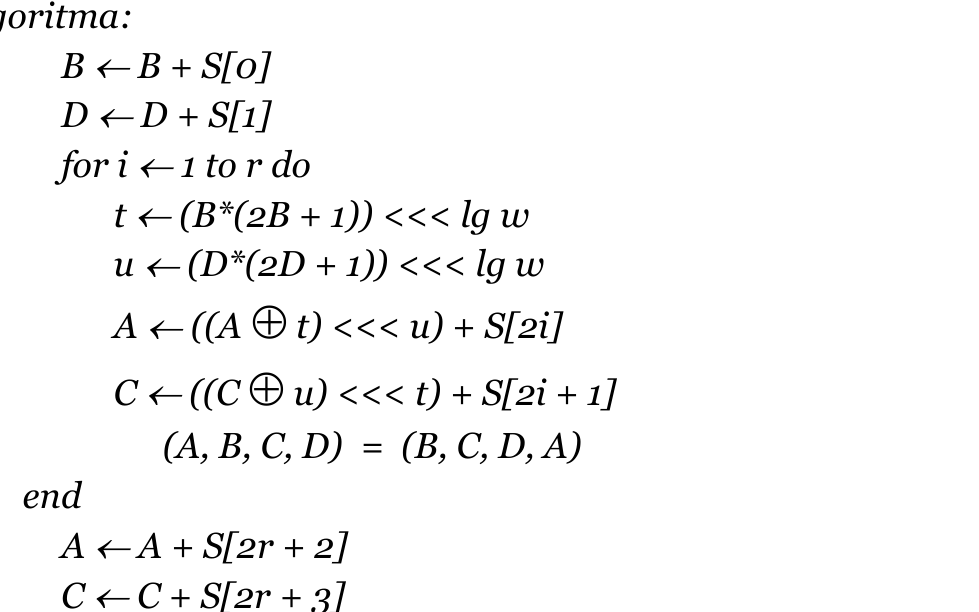
\includegraphics[width=107.10mm,height=168.40mm]{../../images/llm/page_025_img_01.png}%
\end{textblock*}

\end{document}
